\section{Architecture}


Here, we introduce the architecture of the current version of PostgreSQL.
%
We also show how the architecture looks after the refactoring and implementation of the new algorithm.
%
\subsection{Current architecture}
%
In the current version of PostgreSQL the access control module is not identifiable as a stand-alone module in the backend code of the DBMS.
%
Figure~\ref{figure:postgresql:architecture} shows a flowchart of a PostgreSQL server instance.
%
The flowchart shows the backend's behaviour.
%
\subsubsection{Backend architecture}
%
Each box in the flowchart represents a module of PostgreSQL.

The \emph{Main} module is responsible for checking the underlying system requirements, such as the system user starting the server, available memory etc. If all the requirements are met the {Postmaster} process is started.

The \emph{Postmaster} is the starting point for any PostgreSQL server instance. 
%
In this module, system setup tasks such as loading the data representing the database and setting up listeners for database connections are executed.
%
After setting everything up, the Postmaster waits for a connection request from a \emph{frontend application}, i.e., any application that connects to the database.
%
When receiving a connection request, the Postmaster forks itself.
%
The child process then will either authorize the request and become a \emph{Backend} or reject the request and exit.
%
All the blue boxes in the flowchart represent modules of the Backend of a PostgreSQL server.

The Backend consists of an infinite loop that breaks at the parser stage.
%
At this point the Backend is ready to receive a query from the connected frontend application.
%
After receiving a query in text form, the parser creates the abstract syntax tree representing the query.
%
The abstract syntax tree is then passed to the \emph{Traffic Cop}.

The Traffic Cop first analyzes the query to classify it either as a {utility query} or {non-utility query}.
%
\emph{Utility queries} modify the structure of the database, e.g., they create or drop a table, view, or  trigger.
%
\emph{Non-utility queries}, instead, act on the data inside the database.
%
For instance, \texttt{SELECT}, \texttt{DELETE}, and \texttt{UPDATE} are all non-utility queries. 
%
After determining the type, the Traffic Cop forwards utility queries to the \emph{Utility Command} module, which checks the authorization of the query and, if the query is authorized, executes it.

Non-utility commands are forwarded to the \emph{Rewrite Query} module.
%
Here the query is rewritten according to the \emph{PostgreSQL Rule System}.
%
The PostgreSQL Rule System is a collection of rules on how to rewrite queries in such a way that the other modules of the Backend can optimize the query as good as possible.
The Rule System, for instance, expands views to their respective definition, allowing the Generate Paths module to produce more comprehensive execution paths.
%
After the rewriting, the rewritten query is passed to the \emph{Generate Paths} module.
%
Here the system generates different \emph{paths} to execute the query.
%
Each path represents a way of executing the query, i.e., a possible way of traversing the abstract syntax tree.
%
According to internal rules the system will choose the optimal path.
%
This path is passed to the \emph{Generate Plan} module, which internally will generate a \emph{plan} for the executor.
%
A plan is detailed guide for the executor on how to retrieve the tuples.

This plan is then forwarded to the executor, which will execute it and return the tuples to the frontend application.
%
\subsubsection{Access Control}
%
Access control decisions can be made in any of the the following modules: Traffic cop, Executor, or in the module that handles the utility queries.
%
The functions making these decisions, however, also prepare the system for the upcoming change, by, for instance, returning the address where a new table is allocated.
%
Due to the distribution and inconsistency of the access control mechanism, there is no uniform interface that can be called for such a decision.
%
Furthermore,  the mechanism is, sometimes, closely connected to the internals of the database, making the implementation of a new mechanism nearly impossible without refactoring the code.
%
For instance, checking the authorization of \texttt{SELECT} queries is done very late, namely in the executor.
%
This check is on an internal datastructure that represents the tables referenced in the query.
%
Therefore, we need to modify the behaviour of the executor just to modify the way \texttt{SELECT} queries are authorized.
%
This fact motivated us to refactor PostgreSQL in a way that allows for the implementation of new access control mechanisms, without interfering with the internals of the DBMS.

\newpage
%
\begin{figure}[!ht]
  \centering
    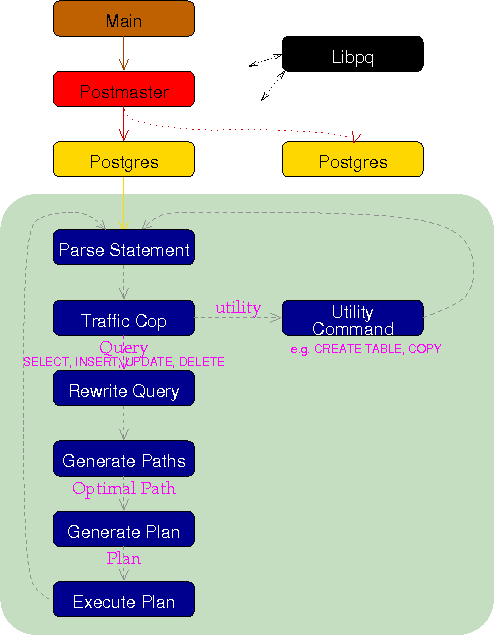
\includegraphics[width=1\textwidth]{img/backend_flowchart.png}
    \caption{Backend Flowchart PostgreSQL \protect \footnotemark}\label{figure:postgresql:architecture}
\end{figure}
%
\footnotetext{\url{http://www.postgresql.org/developer/backend}}
%
\FloatBarrier

%
\subsection{Refactoring}
%
After analyzing the backend, by executing each type of query and following the backend through the process with a debugger, all the functions or code regions relevant to making access control decisions were identified.
%
This identification allowed us to gradually move the code to an external module and build a uniform interface, which is called inside the Traffic cop, when the backend expects a access control decision. 

During the building of this interface we made several design choices.
%
The first decision was to create a stand-alone module in the backend of PostgreSQL dedicated to access control.
This allows developers to clearly identify the code that is responsible for authorizing any type of query.
%
Second we built an interface, that can be called from any module, when requiring an access control decision.

The interface looks as follows:
%
\begin{lstlisting}[frame=single, style=customc]
ac_return_data authorized(ac_decision_data *decision_data);
\end{lstlisting}
%
The structs used in the interface are extensible. For each type of query there is a field in both structs, which represent the input and output data for the all queries of this type.
%
Each field in the decision data struct corresponds to a function that was migrated to the new module.
%
The fields in the decision data struct are pointers to further structs that represent the argument list of the respective function.
%
The structs look as follows: 
%
\begin{lstlisting}[frame=single, style=customc]
union ac_return_data_struct {
	/* Returned if CREATE is authorized otherwise NULL*/
	Oid target_namespace; 
	/* Returned if GRANT is authorized otherwise NULL*/
	AclMode current_privileges; 
	/* Returned for Non-utility query */
	bool execute; 
};

struct ac_decision_data_struct {
	/* Tag identifying query */
	command_type command;
	/* If (command == CREATE_RELATION) this cannot be NULL */
	ac_create_relation_data *create_relation_data; 
	/* If (command == GRANT || command == REVOKE) this cannot be NULL */
	ac_grant_data *grant_data; 
	/* If (command == INSERT || command == DELETE || command == SELECT) this cannot be NULL */
	ac_nutility_data *nutility_data; 
	/* If (command == CREATE_TRIGGER) this cannot be NULL */
	ac_create_trigger_data *create_trigger_data; 
};
\end{lstlisting}
%
Each field in the decision data struct is actually a pointer that refers to a struct, which in turn holds all information needed for deciding if the respective type of query is authorized.
%
For instance, the struct that is required to check the authorization of \texttt{GRANT} or \texttt{REVOKE} queries looks as follows:
%
\begin{lstlisting}[frame=single, style=customc]
/* Data needed for deciding on GRANT queries */
struct ac_grant_data_struct {
	bool is_grant;
	AclMode avail_goptions;
	bool all_privs;
	AclMode privileges;
	Oid objectId;
	Oid grantorId;
	AclObjectKind objkind;
	const char *objname;
	AttrNumber att_number;
	const char *colname;
};
\end{lstlisting}
%
This structure actually represents the argument list of the original function that authorizes \texttt{REVOKE} and \texttt{GRANT} queries.
%
Any function that calls this interface will pass all the data needed to make the decision.
%
Depending on the data received, the interface internally calls the functions that were previously distributed among the modules.
%
This allows future developers to gradually implement a new algorithm, by identifying the query received, and either return the result of a new algorithm, or call the original function responsible for the query.
%
To facilitate the identification of the received query,  we have included an additional field in the decision data, which tells exactly what type of query was received by the interface, e.g., \texttt{INSERT} or \texttt{UPDATE} instead of just identifying it as a non-utility query.

We also added a stack that, at any point of the execution of the database system, holds all queries that are not yet completed, meaning they were not yet interrupted by the access control mechanism nor have they returned any tuples to the frontend application.
%
This allows developers to always have a clear view on the state of the database system.
%
The top element of the stack represents the currently executing query.
%
Elements are popped from the stack after the query is completed.
%
The Backend process consists of one thread, further it is the only process that accesses the context stack, therefore it does not have to be thread-safe.
% 
Each stack's element is a struct that looks as follows:
%
\begin{lstlisting}[frame=single, style=customc]
/* Data structure representing context */
struct ac_context_struct{
	Oid user;
	Oid invoker;
	Query *query;
	const char *query_string;
	bool authorized;
	bool rewritten;
	bool authorizesnext;
};
\end{lstlisting}
%
Each context contains the session user that is connected to the database and the \emph{invoker} of the query.
%
The invoker is relevant if the query is executed under other privileges than the ones of the session user, this happens for instance when a trigger is executed under \emph{owner's privileges}, which means under the privileges of the user that created the trigger.
%
A context also contains the query in text form and as a parsed abstract syntax tree.
%
Also we included three boolean values: ``authorized'' indicates if the query is authorized, ``rewritten'' tells us if the query was rewritten as part of the access control mechanism, and ``authorizesnext'' is used if the query authorizes the query that is below in the context stack. 
%
The fields ``rewritten'' and ``authorizesnext'' are used by our algorithm.
%
The field ``rewritten'' is set to $\top$ after our algorithm has rewritten a query and submits it to the database. 
%
Since the rewritten query is processed the same way as any other query, we need this field prevent the access control mechanism to rewrite the query again.
%
Further the result obtained from the rewritten query will determine the decision if the original query is authorized.
%
More details on the authorization and rewriting of queries will be given in Chapter 5.
%
The stack is used to simplify the implementation of novel mechanisms such as the one in~\cite{guarnieri2016strong}, since the algorithm from Guarnieri et. al requires knowledge about other aspects of the system such as triggers being executed, or nested queries.
%
After the process of refactoring it is possible to integrate any access control mechanism as a plug-in.